\chapter{Unbounded Arrays}
\label{ch:ubarrays}

\newcommand{\lecnum}{11}
%\newcommand{\lectitle}{Unbounded Arrays}
\newcommand{\lecturer}{Rob Simmons, Frank Pfenning}

\chapterTAGS{amortized-cost, array, complexity, correctness, ds-invariant, safety}
\maketitle

\begin{preamble}
\noindent
Arrays have efficient $O(1)$ access to elements given an index, but
their size is set at allocation time.  This makes storing an unknown
number of elements problematic: if the size is too small we may run
out of places to put them, and if it is too large we will waste
memory.  Linked lists do not have this problem at all since they are
extensible, but accessing an element is $O(n)$.  In this lecture, we
introduce \emph{unbounded arrays}, which like lists can hold an
arbitrary number of elements, but also allow these element to be
retrieved in $O(1)$ time?  What gives?  Adding (and removing) an
element to the unbounded array has cost either $O(1)$ or $O(n)$, but
in the long run the average cost of each such operation is constant
--- the challenge will be to prove this last statement!
\end{preamble}

\begin{gram}[Learning Goals]
This maps to our learning goals as follows
\begin{description}
\item[Programming: ]%
  We introduce \emph{unbounded arrays} and operations on them.
\item[Algorithms and Data Structures: ]%
  Analyzing them requires \emph{amortized analysis}, a particular way to
  reason about sequences of operations on data structures.
\item[Computational Thinking: ]%
  We also briefly talk again about \emph{data structure invariants} and
  \emph{interfaces}, which are crucial computational thinking concepts.
\end{description}
But first, let's introduce the idea of amortized analysis on a simpler
example.
\end{gram}


\section{The $n$-bit Counter}
\label{sec:ubarrays:counter}
\TAGS{amortized-cost, complexity}

A simple example we use to illustrate amortized analysis is the idea
of a \emph{binary counter} that we increment by one at a time. If we
have to flip each bit individually, flipping $n$ bits takes $O(n)$
time.
\begin{center}
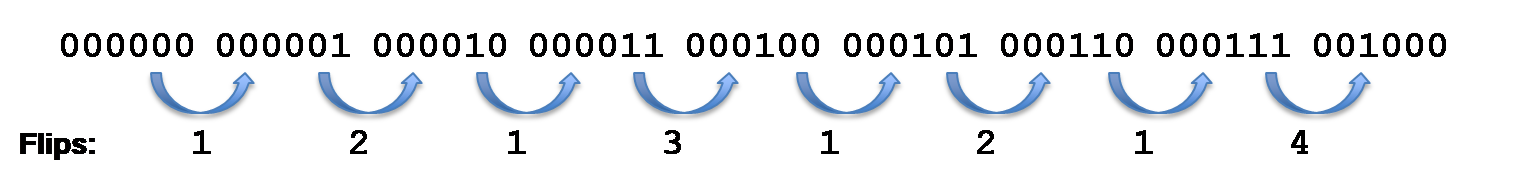
\includegraphics[width=0.99\textwidth]{img/bincount1.png}
\end{center}
Obviously, if we have an $n$-bit counter, the worst case running time
of an single increment operation is $O(n)$. But does it follow that
the worst case running time of $k$ operations is $O(kn)$? Not
necessarily. Let's look more carefully at the cases where the
operation we have to perform is the \emph{most expensive operation
  we've yet considered:}
\begin{center}
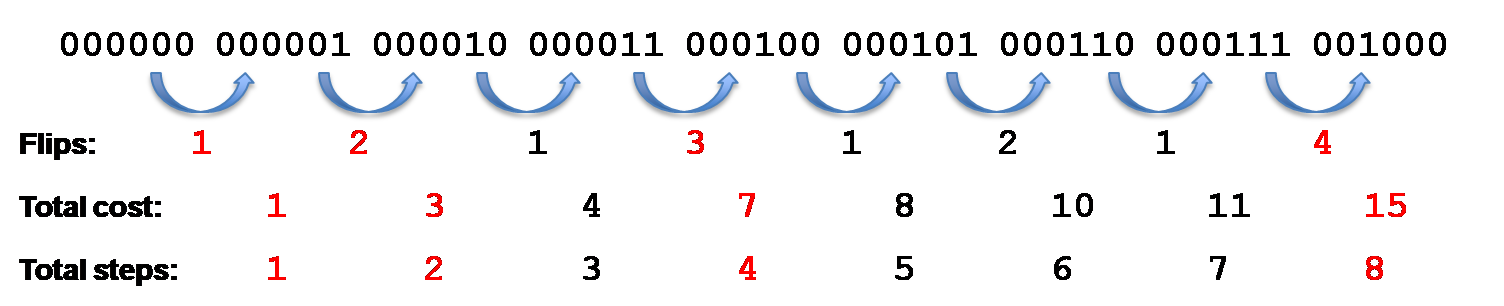
\includegraphics[width=0.99\textwidth]{img/bincount2.png}
\end{center}
We can observe two things informally. First, the most expensive
operations get further and further apart as time goes on. Second,
whenever we reach a most-expensive-so-far operation at step $k$, the
total cost of all the operations up to and including that operation is
$2k-1$. Can we extend this reasoning to say that the total cost of
performing $k$ operations will never exceed $2k$?

One metaphor we frequently use when doing this kind of analysis is
banking.  It's difficult to think in terms of savings accounts full of
microseconds, so when we use this metaphor we usually talk about
\emph{tokens}, representing an abstract notion of cost. With a token,
we can pay for the cost of a particular operation; in this case, the
constant-time operation of flipping a bit. If we \emph{reserve (or
  budget) two tokens} every time we perform any increment, putting any
excess into a savings account, then we see that after the expensive
operations we've looked out, our savings account contains 1 token.
Our savings account appears to never run out of money.

\begin{center}
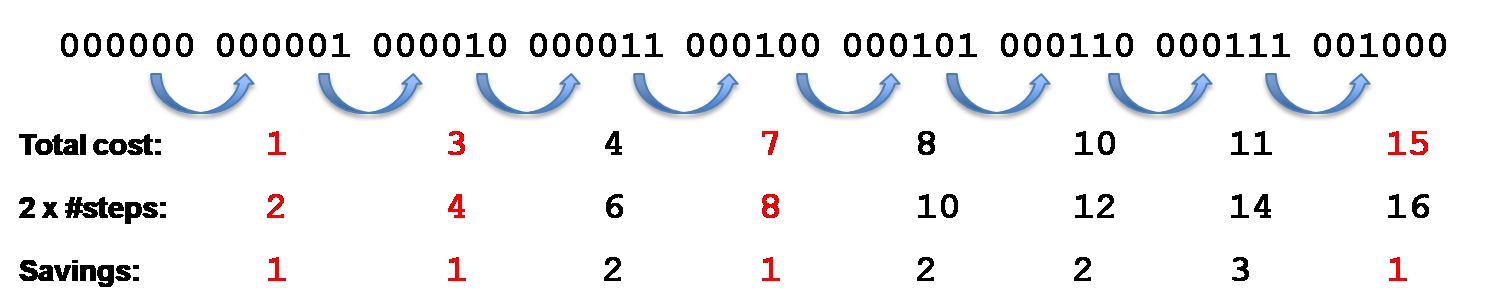
\includegraphics[width=0.99\textwidth]{img/bincount3.png}
\end{center}
This is good evidence, but it still isn't a proof. To offer something
like a proof, as always, we need to talk in terms of
\emph{invariants}. And we can see a very useful invariant: the number
of \lstinline'1' bits always matches the number in our savings
account!  This observation leads us to the last trick that we'll use
when we perform amortized analysis in this class: we associate one
token with each \lstinline'1' in the counter as part of a \emph{meta
  data structure invariant}.  Like normal data structure invariants,
this meta data data structure invariant should hold before and after
carrying out an operation on the data structure.  Differently from
normal data structure invariants, it is not captured in code --- it
resides in our minds only.


\section{Amortized Analysis With Data Structure Invariants}
\label{sec:ubarrays:potential_method}
\TAGS{amortized-cost, complexity}

Whenever we increment the counter, we'll always flip some number
(maybe zero) of lower-order \lstinline'1''s to \lstinline'0', and then
we'll flip exactly one \lstinline'0' to \lstinline'1' (unless we're
out of bits in the counter).  For example, incrementing the 8-bit
counter
\lstinline'10010'\textcolor{red}{\lstinline'0'}\textcolor{blue}{\lstinline'11'}
yields
\lstinline'10010'\textcolor{red}{\lstinline'1'}\textcolor{blue}{\lstinline'00'}:
the two rightmost \textcolor{blue}{\lstinline'1'}'s got flipped to
\lstinline'0''s, the rightmost \textcolor{red}{\lstinline'0'} was
flipped into a \lstinline'1', and all other bits were left unchanged.
We can explain budgeting two tokens for each increment as follows: one
token is used to pay for flipping the rightmost
\textcolor{red}{\lstinline'0'} in the current operation, and one token
is saved for when the resulting \textcolor{blue}{\lstinline'1'} will
need to be flipped into a \lstinline'0' as part of a future increment.
So, how do we pay for flipping the rightmost
\textcolor{blue}{\lstinline'1'}'s in this example?  By using the
tokens that were saved when they got flipped from a \lstinline'0'
into the current \textcolor{blue}{\lstinline'1'}.

No matter how many lower-order \lstinline'1' bits there are, the
flipping of those low-order bits is paid for by the tokens associated
with those bits.  Then, because we're always gaining 2 tokens whenever
we perform an increment, one of those tokens can be used to flip the
lowest-order \lstinline'0' to a \lstinline'1' and the other one can be
associated with that new \lstinline'1' in order to make sure the data
structure invariant is preserved. Graphically, \emph{any} time we
increment the counter, it looks like this:
\begin{center}
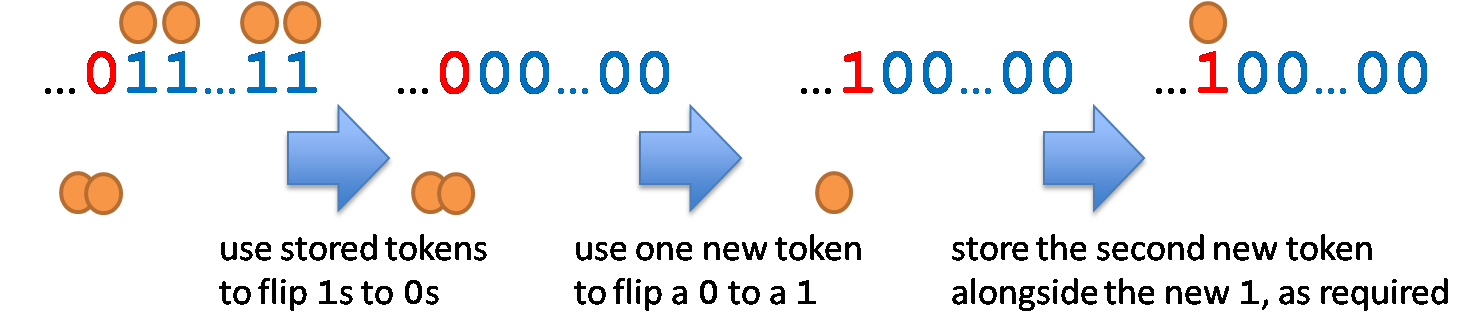
\includegraphics[width=0.9\textwidth]{img/bincount4.png}
\end{center}
(Well, not every time: if the counter is limited to $n$ bits and
they're all \lstinline'1', then we'll flip all the bits to
\lstinline'0'. In this case, we can just throw away or lose track of
our two new tokens, because we can restore the data structure
invariant without needing the two new tokens. In the accounting or
banking view, when this happens we observe that our savings account
now has some extra savings that we'll never need.)

Now that we've rephrased our operational argument about the amount of
savings as a data structure invariant that is always preserved by the
increment operation, we can securely say that, each time we increment
the counter, it suffices to reserve exactly two tokens. This means
that a series of $k$ increments of the $n$-bit counter, starting when
the counter is all zeroes, will take time in $O(k)$. We can also say
that each individual operation has an \emph{amortized running time} of
2 bit flips, which means that the \emph{amortized} cost of each
operation is in $O(1)$. It's not at all contradictory for bit flips to
have an amortized running time in $O(1)$ and a worst-case running time
in $O(n)$.

In summary: to talk about the amortized running time (or, more
generally, the amortized \emph{cost}) of operations on a data
structure, we:
\begin{enumerate}
\item%
  Invent a notion of \emph{tokens} that stand in for the resource that
  we're interested in (usually time --- in our example, a token is
  spent each time a bit is flipped);
\item%
  Specify, for any instance of the data structure, how many tokens
  need to be held in reserve as part of the data structure invariant
  (in our example, one token for each 1-bit);
\item%
  Assign, for each operation we might perform on the data structure,
  an amortized cost in tokens (in our example, two tokens for each
  increment);
\item%
  Prove that, for any operation we might perform on the data
  structure, the amortized cost plus the tokens held in reserve as
  part of the data structure invariant suffices to restore the data
  structure invariant.
\end{enumerate}
This analysis proves that, for any \emph{sequence} of operations on a
data structure, the cumulative cost of that sequence of operations
will be less than or equal to the sum of the amortized cost of those
operations. Even if some of the operations in that sequence have high
cost (take a long time to run), that will be at least paid for by
other operations that have low cost (take a short time to run).

This form of amortized analysis is sometimes called the
\emph{potential method}. It is a powerful mathematical technique, but
we'll only use it for relatively simple examples in this class.


\section{What amortized analysis means}
\label{sec:ubarrays:theory}
\TAGS{amortized-cost, complexity}

Tokens aren't real things, of course! They are stand-ins for the
actual resources we're interested in. Usually, the resource we are
concerned about is time, so we match up tokens to the (frequently
constant-time) operations we have to do on our data structure. In the
current example, we might be storing the counter as an array of
\lstinline'bool' values, in which case it would take a constant-time
array write to flip one of the bits in the counter. (Tokens will also
correspond to array writes in the unbounded array example we consider
next.)

We do amortized analysis in order to prove that the
\emph{inexpensive operations early on} suffice to pay for
\emph{any expensive operations} that happen later. There's no
uncertainty with amortized analysis: we know that, if we calculate our
overall time as if each increment costs two bit flips, we will never
underestimate the total cost of our computation.
\begin{center}
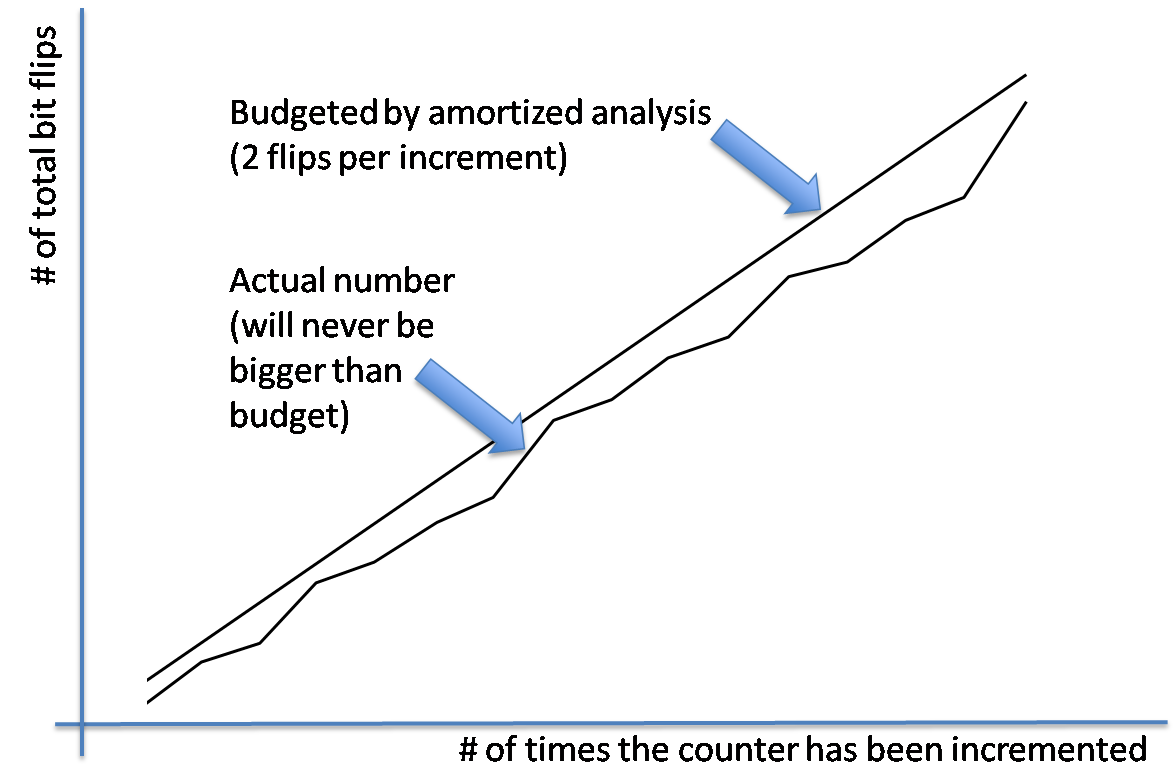
\includegraphics[width=0.75\textwidth]{img/bitflip-graph.png}
\end{center}

This is different than average case analysis for quicksort, where we
know that sometimes the total cost of sorting could be higher than
predicted (if we get unlucky in our random pivot selection). There's
no luck in our amortized analysis: we know that the total cost of $k$
increments is in $O(k)$, even though the worst case cost of a single
increment operation is $O(n)$ bit flips.


\section{Unbounded Arrays}
\label{sec:ubarrays:arrays}
\TAGS{amortized-cost, array, complexity}

In a previous homework assignment, you were asked to read in some
files such as the \emph{Collected Works of Shakespeare}, the
\emph{Scrabble Players Dictionary}, or anonymous tweets collected from
Twitter.  What kind of data structure do we want to use when we read
the file?  In later parts of the assignment we want to look up words,
perhaps sort them, so it is natural to want to use an array of
strings, each string constituting a word.  A problem is that before we
start reading we don't know how many words there will be in the file
so we cannot allocate an array of the right size!  One solution uses
either a queue or a stack.

A non-sorting variant of the self-sorting array interface that we
discussed before doesn't seem like it would work, because it requires
us to bound the size of the array --- to know in advance how much data
we'll need to store.  Let's call this unsorted variant
\lstinline'uba_t' and rename the rest of the interface accordingly:
\begin{lstlisting}[language={[C0]C}]
// typedef ______* uba_t;

int uba_len(uba_t A)
  //@requires A != NULL;
  //@ensures \result >= 0;
;

uba_t uba_new(int size)
  //@requires 0 <= size;
  //@ensures \result != NULL;
  //@ensures uba_len(\result) == size;
;

string uba_get(uba_t A, int i)
  //@requires A != NULL;
  //@requires 0 <= i && i < uba_len(A);
;

void uba_set(uba_t A, int i, string x)
  //@requires A != NULL;
  //@requires 0 <= i && i < uba_len(A);
;
\end{lstlisting}
It would work, however, if we had an extended interface of
\emph{unbounded arrays}, where the \lstinline'uba_add(A,x)' function
increases the array's size to add \lstinline'x' to the end of the
array. There's a complementary operation, \lstinline'uba_rem(A)', that
decreases the array's size by 1.

\clearpage
\begin{lstlisting}[language={[C0]C}]
void uba_add(uba* A, string x)
  //@requires A != NULL;
;

string uba_rem(uba* A)
  //@requires A != NULL;
  //@requires 0 < uba_len(A);
;
\end{lstlisting}
We'd like to give all the operations in this extended array interface
a running time in $O(1)$.\footnote{It's questionable at best whether
  we should think about
  \lstinline[basicstyle=\smallerbasicstyle]'uba_new' being $O(1)$,
  because we have to allocate $O(n)$ space to get an array of length
  $n$ and initialize all that space to default values. The operating
  system has enough tricks to get this cost down, however, that we
  usually think of array allocation as a constant-time operation.}
It's not practical to give \lstinline'uba_add(A,x)' a worst case
running time in $O(1)$, but with a careful implementation we can show
that is possible to give the function an \emph{amortized} running time
in $O(1)$.

%% We'll extend this data structure with


%%  We then have to prove that, for any such operation, the new
%% tokens associated with the amortized


%% we perform on this data structure, the amortized cost (in tokens) of that
%% operation, combined with the number of tokens held in savings as part of the data structure invariant.

%% that we associate with the data structure as part of the

%% Questions:




%% \paragraph{Note For Summer 2014:} This interface and implementation of unbounded arrays described here
%% is a bit different than the one in class and posted to
%% \url{http://www.cs.cmu.edu/~rjsimmon/15122-m14/lec/10-ubarrays/arr.c0}. The
%% most important differences are:
%% \begin{itemize}
%% \item Our arrays were named \lstinline'uba_', these are named \lstinline'uba_'.
%% \item We gave an initial \emph{size} to our array (and arrays are
%%   initialized in the usual C0 fashion like all other heap-allocated
%%   memory), the interface here starts arrays at size 0 and gives them
%%   an initial limit (a part of the implementation that
%%   shouldn't necessarily be available to the programmer!)
%% \item Our data structure invariant required that the size be strictly
%%   less than the limit, which had the result that we always wasted one
%%   cell of the array. This changed amortized analysis a little bit, but
%%   the result is the same.
%% \end{itemize}

%% \section{Unbounded Arrays}

%%   We discussed this in Lectures 9 on queues and
%% stacks.
%%   .

%% Thinking about it abstractly, an unbounded array should be like an
%% array in the sense that we can get and set the value of an arbitrary
%% element via its index $i$.  We should also be able to add a new
%% element to the end of the array, and delete an element from the end of
%% the array.

%% We use the unbounded array by creating an empty one before reading a
%% file.  Then we read words from the file, one by one, and add them to
%% the end of the unbounded array.  Meanwhile we can count the number of
%% elements to know how many words we have read.  We trust the data
%% structure not to run out of space unless we hit some hard memory
%% limit, which is unlikely for the kind of task we have in mind, given
%% modern operating systems.  When we have read the whole file the
%% words will be in the unbounded array, in order, the first word
%% at index $0$, the second at index $1$, etc.

%% The general implementation strategy is as follows.  We maintain an
%% array of a fixed length $\mathit{limit}$ and an internal index
%% $\mathit{size}$ which tracks how many elements are actually used in the
%% array.  When we add a new element we increment $\mathit{size}$, when
%% we remove an element we decrement $\mathit{size}$.  The tricky issue
%% is how to proceed when we are already at the limit and want to add
%% another element.  At that point, we allocate a new array with a larger
%% limit and copy the elements we already have to the new array.  For
%% reasons we explain later in this lecture, every time we need to
%% enlarge the array we \emph{double} its size.  Removing an element
%% from the end is simple: we just decrement $\mathit{size}$.  There
%% are some issues to consider if we want to shrink the array, but
%% this is optional.

%% \section{An Interface to Unbounded Arrays}

%% As usual when designing a data structure, we start by thinking about
%% its interface.  We must be able to create a new unbounded array,
%% access its elements (both for reading and writing), and add or remove
%% elements at the end.  The elements of the array should be of arbitrary
%% type (like ordinary arrays), but we cannot achieve this form of
%% genericity in C0 at present.  We will discuss ways to write generic
%% code later in the course when we move to C\@.  Instead, we just
%% indicate this by defining and using a type name \lstinline'elem' (here as
%% \lstinline'string').  These considerations lead us to the following
%% interface:

%% \begin{lstlisting}[language={[C0]C}]
%% typedef string elem;

%% /* Interface of unbounded arrays */

%% typedef struct uba_header* uba;

%% uba uba_new(int initial_limit)
%% //@requires initial_limit > 0;
%%   ;

%% int uba_size(uba L)               /* "\length(L)" */
%% //@ensures \result >= 0;
%%   ;

%% elem uba_get(uba L, int index)    /* "L[index]" */
%% //@requires 0 <= index && index < uba_size(L);
%%   ;

%% void uba_set(uba L, int index, elem e)  /* "L[index] = e" */
%% //@requires 0 <= index && index < uba_size(L);
%%   ;

%% void uba_add(uba L, elem e);      /* add e at the end of L */

%% elem uba_rem(uba L)               /* remove last element in L */
%% //@requires uba_size(L) > 0;
%%   ;
%% \end{lstlisting}

%% Contracts on interfaces are cumulative with respect to the contracts
%% on the implementations: both are checked when a function is called
%% through its interface.  Note that we do not mention \lstinline'is_uba',
%% since this function is not exposed to the client.  Client code should
%% only ever be able to obtain valid unbounded arrays if it uses the
%% interface, so preservation of the data structure invariants should be
%% considered an \emph{internal invariant} of the data structure
%% implementation.

%% Please read over the interface carefully to make sure you understand
%% all of its provisions.  We would like all the specified operations to
%% take only \emph{constant time}, that is, $O(1)$.  As we will see in
%% the remainder of this lecture this is quite tricky and we have to make
%% some intriguing qualifications in our statement of the asymptotic
%% complexity.

%% Unfortunately, C (and, by association, C0) does not provide a way to
%% enforce that clients do not incorrectly exploit details of the
%% implementation of a data structure.  Higher-level languages such as
%% Java or ML have interfaces and data abstraction as one of their
%% explicit design goals.  In this course, the use of interfaces is a
%% matter of programming discipline.  As we discuss further data
%% structures we generally focus on the interface first, before writing
%% any code.  This is because the interface often guides the selection
%% of an implementation technique and the individual functions.


\section{Implementing Unbounded Arrays}
\label{sec:ubarrays:implementing}
\TAGS{amortized-cost, array, correctness, ds-invariant, safety}

Our original implementation of an interface for self-sorting arrays
had a struct with two fields: the \lstinline'data' field, an actual
array of strings, and a \lstinline'length' field, which contained the
length of the array.  This value, which we will call the \emph{limit}
when talking about unbounded arrays, was what we returned to the users
when they asked for the length of the array.

While it wouldn't work to have a limit that was \emph{less} than the
array length we are reporting to the user, we can certainly have an
array limit that is greater: we'll store the potentially smaller
number that we report in the \lstinline'size' field.
\begin{lstlisting}[language={[C0]C}]
typedef struct uba_header uba;
struct uba_header {
  int size;         /* 0 <= size && size < limit */
  int limit;        /* 0 < limit                 */
  string[] data;    /* \length(data) == limit    */
};
typedef uba* uba_t;

int uba_len(uba* A)
//@requires is_uba(A);
//@ensures 0 <= \result && \result <= \length(A->data);
{
  return A->size;
}
\end{lstlisting}
If we reserve enough extra room, then most of the time when we need to
use \lstinline'uba_add' to append a new item onto the end of the
array, we can do it by just incrementing the \lstinline'size' field
and putting the new element into an already-allocated cell in the
\lstinline'data' array.
\begin{center}
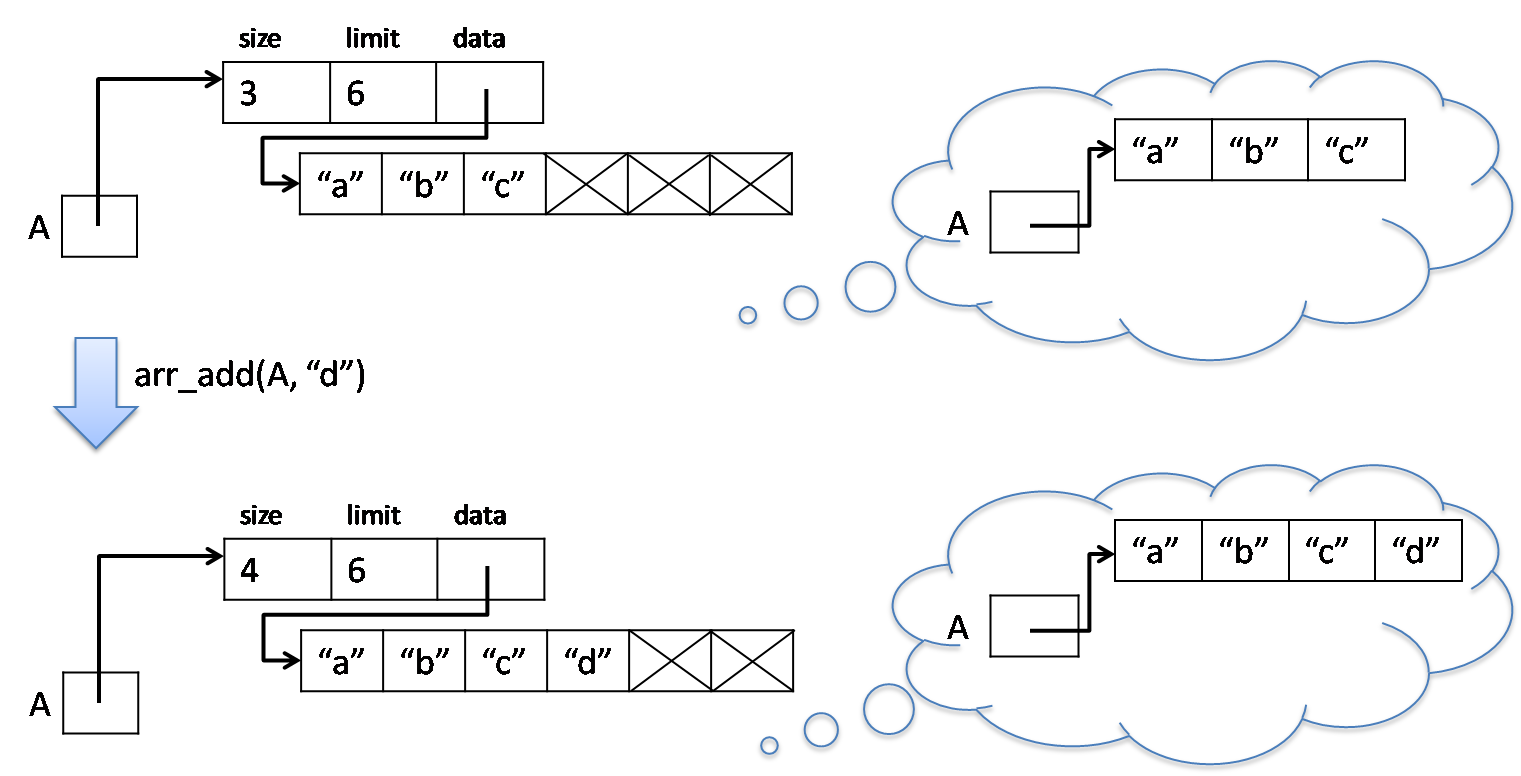
\includegraphics[width=0.99\textwidth]{img/views.png}
\end{center}
The images to the left above represent how the data structure is
actually stored in memory, and the images in the thought bubbles to
the right represent how the client of our array library can think
about the data structure after an \lstinline'uba_add' operation.

The data structure invariant sketched out in comments above can be
turned into an \lstinline'is_uba' function like this:
\begin{lstlisting}[language={[C0]C}]
bool is_uba_expected_length(string[] A, int limit) {
  //@assert \length(A) == limit;
  return true;
}

bool is_uba(uba* A) {
  return A != NULL
    && is_uba_expected_length(A->data, A->limit)
    && 0 <= A->size && A->size < A->limit;
}
\end{lstlisting}
Because we require that the size be strictly less than the limit, we
can always implement \lstinline'uba_add' by storing the new string in
\lstinline'A->data[A->size]' and then incrementing the size. But after
incrementing the size, we might violate the data structure invariant!
We'll use a helper function, \lstinline'uba_resize', to resize the
array in this case.

\begin{lstlisting}[language={[C0]C}]
void uba_add(uba* A, string x)
//@requires is_uba(A);
//@ensures is_uba(A);
{
  A->data[A->size] = x;
  (A->size)++;
  uba_resize(A);
}
\end{lstlisting}
The \lstinline'uba_resize()' function works by allocating a new array,
copying the old array's contents into the new array, and replacing
\lstinline'A->data' with the address of the newly allocated array.

\begin{lstlisting}[language={[C0]C}]
void uba_resize(uba* A)
//@requires A != NULL && \length(A->data) == A->limit;
//@requires 0 < A->size && A->size <= A->limit;
//@ensures is_uba(A);
{
  if (A->size == A->limit) {
    assert(A->limit <= int_max() / 2); // Can't handle bigger
    A->limit = A->size * 2;
  } else {
    return;
  }

  //@assert 0 <= A->size && A->size < A->limit;
  string[] B = alloc_array(string, A->limit);

  for (int i = 0; i < A->size; i++)
  //@loop_invariant 0 <= i && i <= A->size;
  {
    B[i] = A->data[i];
  }

  A->data = B;
}
\end{lstlisting}
The assertion \lstinline'assert(A->limit <= int_max() / 2)' is there
because, without it, we have to worry that doubling the limit in the
next line might overflow. \emph{Hard asserts} like this allow us to
safely detect unlikely failures that we can't exclude with contracts
but that we don't want to encode into our interface.


\section{Amortized Analysis for Unbounded Arrays}
\label{sec:ubarrays:uba_analysis}
\TAGS{amortized-cost, array}

Doubling the size of the array whenever we resize it allows us to give
an amortized analysis concluding that every \lstinline'uba_add'
operation has an amortized cost of \emph{three} array writes. Because
array writes are our primary notion of cost, we say that one token
allows us to write to an array one time.

% Here's how the analysis works: our \emph{data structure invariant} for
% tokens is that, whenever we are using a cell in the \emph{second half
%   of the array}, we need to store two tokens alongside that cell: one
% to copy this cell when we double the array in a future resize and one
% for copying the corresponding cell in the first half of the array at
% that time (why? that cell has been put into use long ago and there was
% no way to predict how many times it would be copied). Thus we assign
% an \emph{amortized cost} of three tokens to the add operation. Every
% call to \lstinline'uba_add' uses one token to write an element into
% the array; if that new element is in the second half of the array, we
% store two tokens alongside that newly-in-use cell. Thus, budgeting
% three tokens for each \lstinline'uba_add' operation suffices to
% preserve the data structure invariant in every case that doesn't cause
% the array to become totally full.
% \begin{center}
% 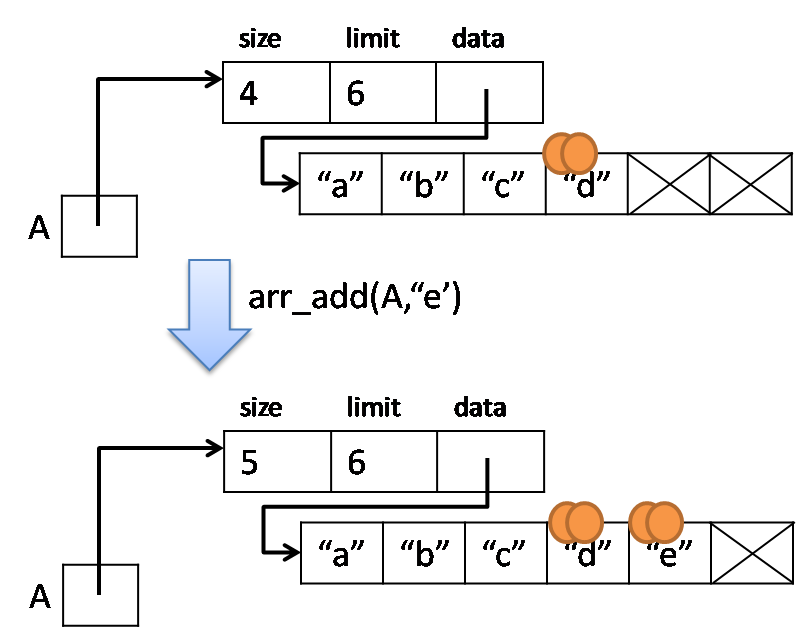
\includegraphics[width=0.6\textwidth]{img/token.png}
% \end{center}

Here's how the analysis works: our \emph{data structure invariant} for
tokens is that every cell in use in the \emph{second half of the
  array} (i.e., each cell at index $i$ in $\lbrack \mathit{limit}/2,
\mathit{size})$) and the corresponding cell in the first half of the
array (at index $i - \mathit{limit}/2$) will have one token associated
with it.  For clarity, we color tokens in the first half of the array
in blue and tokens in the second half in gold.
Each time we add an element to the array (at index
$\mathit{size}$), we use one token to perform that very write, store
one gold token with this element for copying it next time we double the
size the array in a future resize, and store one blue token for copying the
corresponding element in the first half of the array (at index
$\mathit{size} - \mathit{limit}/2$) on that same resize.  Thus,
budgeting three tokens for each \lstinline'uba_add' operation suffices
to preserve the data structure invariant in every case that doesn't
cause the array to become totally full.  We therefore assign an
\emph{amortized cost} of three tokens to the add operation.
\begin{center}
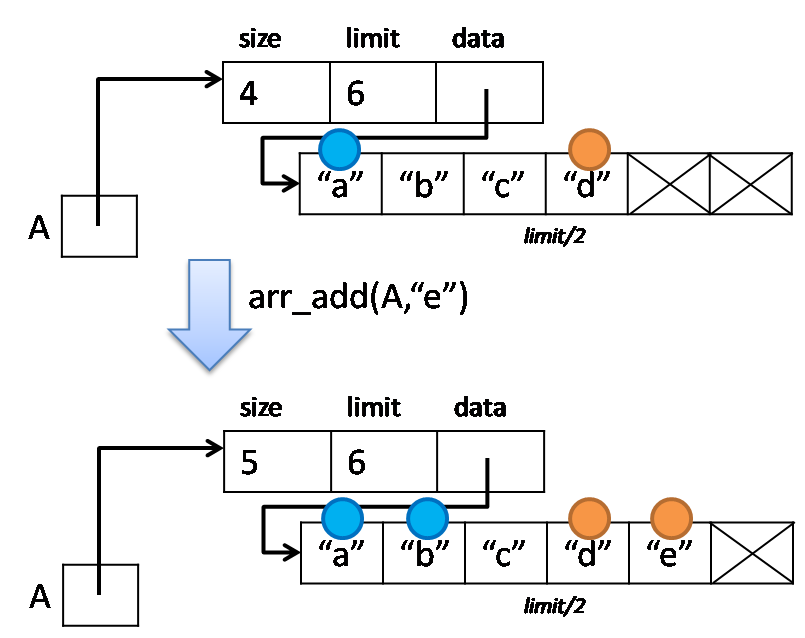
\includegraphics[width=0.6\textwidth]{img/tokenB.png}
\end{center}

In the cases where the addition does completely fill the array, we
need to copy over every element in the old array into a new, larger
array in order to preserve the \lstinline'A->size < A->limit' data
structure invariant.  This requires one write for every element in the
old array.  We can pay for each one of those writes because we now
have one gold token for each element in the second half of the old array
(at indices $\lbrack \mathit{limit}/2, \mathit{limit})$) and one blue token for
each element in the first half of that array (at indices $\lbrack 0,
\mathit{limit}/2)$) --- which is the same as having one token for each
cell in the old array.
\begin{center}
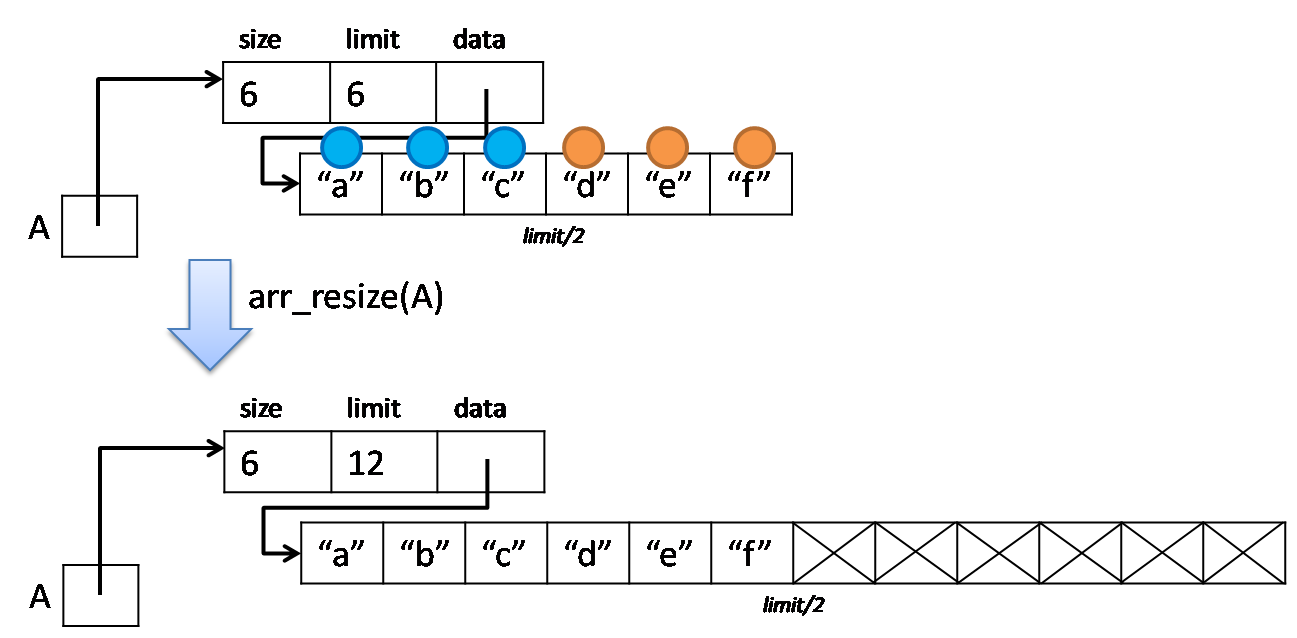
\includegraphics[width=0.99\textwidth]{img/doubleB.png}
\end{center}
After the resize, exactly half the array is full, so our data
structure invariant for tokens doesn't require us to have any tokens
in reserve. This means that the data structure invariant is preserved
in this case as well.  In general, the number of tokens associated
with an unbounded array is $2\times\mathit{size} - \mathit{limit}$.

This establishes that the amortized cost of \lstinline'uba_add' is
three array writes.  We do things that aren't array writes in the
process of doing \lstinline'uba_add', but the cost is dominated by
array writes, so this gives the right big-O notion of (amortized)
cost.

\section{Shrinking the array}
\label{sec:ubarrays:shrinking}
\TAGS{amortized-cost, array}

In the example above, we only resized our array to make it bigger. We
could also call \lstinline'uba_resize(A)' in our \lstinline'uba_rem'
function, and allow that function to make the array either bigger or
smaller.

\begin{lstlisting}[language={[C0]C}]
string uba_rem(uba* A)
//@requires is_uba(A);
//@requires 0 < uba_len(A);
//@ensures is_uba(A);
{
  (A->size)--;
  string x = A->data[A->size];
  uba_resize(A);
  return x;
}
\end{lstlisting}

If we want \lstinline'uba_rem' to take amortized constant time, it
will not work to resize the array as soon as \lstinline'A' is less
than half full. An array that is exactly half full doesn't have any
tokens in reserve, so it wouldn't be possible to pay for halving the
size of the array in this case. In order to make the constant-time
amortized cost work, the easiest thing to do is only resize the array
when it is less than \emph{one-quarter} full.  If we make this change,
it's possible to reflect it in the data structure invariant, requiring
that \lstinline'A->size' be in the range $\lbrack $\lstinline'A->limit/4',
\lstinline'A->limit') rather than the range $\lbrack 0$,
\lstinline'A->limit') that we required before.

In order to show that this deletion operation has the correct
amortized cost, we must extend our data structure invariant to also
store tokens for every unused cell in the left half of the array. (See
the exercises below.) Once we do so, we can conclude that \emph{any}
valid sequence of $n$ operations (\lstinline'uba_add' or
\lstinline'uba_rem') that we perform on an unbounded array will take
time in $O(n)$, even if any single one of those operations might take
time proportional to the current length of the array.

\clearpage
\section{Exercises}
\label{sec:ubarrays:exercises}

\begin{exercise}
  If we only add to an unbounded array, then we'll never have less
  than half of the array full. If we want \lstinline'uba_rem' to be
  able to make the array smaller, we'll need to reserve tokens when
  the array is less than half full, not just when the array is more
  than half full. What is the precise data structure invariant we
  need? How many tokens (at minimum) do we need to per
  \lstinline'uba_rem' operation in order to preserve it? What is the
  resulting amortized cost (in terms of array writes) of
  \lstinline'uba_rem'?
\end{exercise}

\begin{exercise}
  Here's the code for \lstinline'uba_new':
\begin{lstlisting}[language={[C0]C}, numbers=left, firstnumber=53]
uba* uba_new(int size)
//@requires 0 <= size;
//@ensures is_uba(\result);
//@ensures uba_len(\result) == size;
{
  uba* A = alloc(uba);
  int limit = size == 0 ? 1 : size*2;
  A->data = alloc_array(string, limit);
  A->size = size;
  A->limit = limit;

  return A;
}
\end{lstlisting}
Line 59 initializes \lstinline'limit' to 1 if
\lstinline'size' is equal to 0, and to \lstinline'size*2' otherwise
--- do you see why?

  If we also said that we required $n$ tokens to allocate an array of
  size $n$, then the \lstinline'uba_new' function would obviously have
  a cost (amortized and worst-case) of $2n \in O(n)$.  How many tokens
  would we need to budget for each \lstinline'uba_add' and
  \lstinline'uba_rem' operation in order to prove that these
  operations require an amortized constant number of tokens?
\end{exercise}

\begin{exercise}
  How would our amortized analysis change if we increased the size of
  the array by 50\% instead of 100\%? What if we increased it by
  300\%? You are allowed to have a cost in fractions of a token.
\end{exercise}

\begin{exercise}
  When removing elements from the unbounded array we resize if the
  limit grossly exceeds its size. Namely when %
  \lstinline'L->size < L->limit/4'.  %
  Your first instinct might have been to already shrink the array when
  \lstinline'L->size < L->limit/2'.  We have argued by example why
  that does not give us constant amortized cost $O(n)$ for a sequence
  of $n$ operations.  We have also sketched an argument why
  \lstinline'L->size < L->limit/4' gives the right amortized cost.  At
  which step in that argument would you notice that %
  \lstinline'L->size < L->limit/2' %
  is the wrong choice?
\end{exercise}

\begin{exercise}
  When removing elements from the unbounded array we resize if the limit
  grossly exceeds its size. Namely when \lstinline'L->size <= L->limit/4'.
  Your first instinct might have been to already shrink the array when
  \lstinline'L->size <= L->limit/2'.  We have argued by example why that does
  not give us constant amortized cost $O(n)$ for a sequence of $n$ operations.
  We have also sketched an argument why \lstinline'L->size <= L->limit/2'
  gives the right amortized cost.  At which step in that argument would you
  notice that \lstinline'L->size <= L->limit/2' is the wrong choice?
\end{exercise}

% \clearpage
% \bibliographystyle{alpha}
% \bibliography{modal}
